\documentclass[11pt,a4paper]{article}
% ============================================================
% Financial Econometrics group project --- Replication of
% Kozak, Nagel & Santosh (2020) "Shrinking the Cross-Section" (JFE)
% English report. Compile locally with: xelatex report.tex
% (article + xeCJK; xeCJK only renders the Chinese author names.)
% ============================================================
\usepackage{amsmath,amssymb}
\usepackage{graphicx}
\usepackage{booktabs}
\usepackage{geometry}
\usepackage{caption}
\usepackage{float}
\usepackage{array}
\usepackage[hidelinks]{hyperref}
\usepackage{xeCJK}
\geometry{margin=2.4cm}
\captionsetup{font=small,labelfont=bf}

% CJK font only for the Chinese author names (fandol not installed; use AR PL UMing).
\setCJKmainfont{AR PL UMing CN}

\graphicspath{{../outputs/}{../results_export/}}
\newcommand{\Eb}{\mathbb{E}}
\newcommand{\Rtwo}{R^2}

% ===== Privacy: real names / IDs / majors live in the gitignored authors.local.tex =====
% The public repo ships only placeholders; if authors.local.tex exists locally it overrides
% them (template: authors.local.tex.example).
\newcommand{\memberA}{Member A}\newcommand{\sidA}{ID-A}\newcommand{\majorA}{Major A}
\newcommand{\memberB}{Member B}\newcommand{\sidB}{ID-B}\newcommand{\majorB}{Major B}
\IfFileExists{./authors.local.tex}{\input{./authors.local.tex}}{}

\title{\textbf{Shrinking the Cross-Section:\\ A Replication and a Machine-Learning Extension of Kozak, Nagel \& Santosh (2020)}}
\author{\memberA~\sidA \quad \memberB~\sidB \\[2pt]
\small Peking University \quad Financial Econometrics \quad Group 3}
\date{\today}

\begin{document}
\maketitle

\begin{abstract}
\noindent We replicate Kozak, Nagel \& Santosh (2020, \emph{Journal of Financial Economics}; hereafter KNS),
``Shrinking the Cross-Section.'' KNS construct a robust stochastic discount factor (SDF) that shrinks the
contribution of low-variance principal components (PCs) more strongly, and argue that \textbf{L2 (ridge)
shrinkage of the PCs of the universe of anomaly factors far outperforms sparse models that keep only a few
factors}. Under the hard constraints of CPU-only computation, minimal dependencies, and no paid data, we
(i) make the original Python port run and \textbf{reproduce the paper's four core results with a single command};
(ii) carry out an honest machine-learning extension; and (iii) add \textbf{five further extensions and robustness
analyses}: the literal $\eta{=}1$ Pástor--Stambaugh benchmark, a \textbf{generalized shrinkage curve that learns
the shrinkage shape $\eta$}, block-bootstrap confidence intervals, a look-ahead-free train-only PC rotation, and
the FF25 preliminary analysis. The core findings reproduce cleanly: shrinkage is necessary, relative shrinkage is
the key, and sparsity exists only in PC space. The machine-learning extension \textbf{honestly shows that giving
the shrinkage function extra flexibility yields no statistically significant out-of-sample improvement}, confirming
the paper's thesis that pricing information is diffuse and linear relative shrinkage is already near-optimal. All
results reproduce in about two minutes via \texttt{reproduce\_all.py} with fixed random seeds.
\end{abstract}

% ============================================================
\section{Introduction and the paper's core claims}
% ============================================================
The empirical asset-pricing literature has uncovered a large number of stock characteristics that predict the
cross-section of returns. The dominant approach summarizes them with a small number of characteristics-based
factors (e.g.\ the Fama--French three/five factors), i.e.\ it seeks a \textbf{characteristics-sparse} SDF. KNS
question this paradigm: faced with dozens or even thousands of candidate factors, a cross-sectional regression
badly overfits the noise in factor means and performs poorly out of sample. Economics (the absence of near-arbitrage)
implies that any factor earning a substantial risk premium must be a major source of covariance, so pricing
information should be concentrated in \textbf{high-variance principal components}. KNS therefore impose a Bayesian
prior that shrinks SDF coefficients \textbf{increasingly with the eigenvalue}, choosing the hyperparameters by
maximizing the out-of-sample (OOS) cross-sectional $\Rtwo$.

\textbf{The paper's three core claims}, which form our replication backbone:
\begin{enumerate}
  \item \textbf{Shrinkage is necessary, and relative shrinkage is the key.} The naive un-shrunk estimator collapses
  out of sample; equal (level) shrinkage à la Pástor--Stambaugh ($\eta{=}1$) is far worse than relative
  shrinkage ($\eta{=}2$), which shrinks low-variance PCs more aggressively.
  \item \textbf{There is almost no sparsity in characteristics space.} Forcing the SDF to keep only a few raw
  anomaly factors sharply degrades OOS performance --- there is very little redundancy among anomalies.
  \item \textbf{Sparsity exists only in PC space.} A few high-variance PCs already approximate the SDF well, but
  the pricing information is in fact spread over about twenty PCs rather than concentrated in the first few.
\end{enumerate}

\textbf{Our contribution.} On top of lukaskoerber's Python port we (1) fix porting bugs so it runs on
Python 3.14 + pandas 3; (2) reproduce the four core results (Figures 1--4) under a unified pipeline; (3) carry out
a tiny-MLP nonlinear-shrinkage extension (Figure 5); and (4) \textbf{add five extensions} (Figures 6--8 plus a
bootstrap): the literal $\eta{=}1$ benchmark, the generalized shrinkage curve (learning $\eta$), block-bootstrap
confidence intervals, a look-ahead-free rotation, and the FF25 preliminary analysis. Everything is CPU-only,
minimal-dependency, and seed-fixed.

% ============================================================
\section{Data}
% ============================================================
All data are \textbf{portfolio-level returns} or freely available Ken French data; there are \textbf{no paid
sources} (no WRDS / CRSP / Compustat / IBES).
\begin{itemize}
  \item \textbf{50 anomaly long--short portfolios} (the main dataset, \texttt{managed\_portfolios\_anom\_d\_50.csv}):
  daily, 1963-07 to 2017-12, $T\approx 11{,}000$. Each column is the return of a zero-investment long--short
  portfolio sorted on one anomaly characteristic, plus the market excess return \texttt{rme}. This is the
  battleground of the paper's Section 4.2, Figures 3/4, and Table 1.
  \item \textbf{FF25} (25 size/BM portfolios) and the Fama--French factors: freely available from the Ken French
  data library; used in the paper's Section 4.1 as a low-dimensional ``known-answer'' preliminary analysis
  (see extension R1, Section \ref{sec:r1}).
\end{itemize}
Preprocessing (as in the original repo): regress out the market $\beta$ of each column (de-market), then
standardize to the market volatility (de-vol). Hence the factors $F$ are \textbf{market-orthogonalized long--short
portfolios}, and the SDF explains only cross-sectional differences beyond the market.

% ============================================================
\section{Methodology}\label{sec:method}
% ============================================================
\subsection{The SDF and the shrinkage prior}
We seek an SDF in the span of returns (Hansen--Jagannathan):
\begin{equation}
  M_t = 1 - b'\big(F_t - \Eb[F_t]\big),\qquad \Eb[M_t F_t]=0
  \;\Rightarrow\; b = \Sigma^{-1}\Eb[F_t],
\end{equation}
where $\Sigma=\operatorname{Cov}(F_t)$. The naive sample estimator $\hat b=\bar\Sigma^{-1}\bar\mu$ badly overfits
the noise in the means in high dimensions. Rotating to principal components, $\Sigma=QDQ'$,
$D=\operatorname{diag}(d_1,\dots,d_N)$ (eigenvalues in decreasing order), $P_t=Q'F_t$, KNS impose the prior family
\begin{equation}
  \mu \sim \mathcal{N}\!\Big(0,\ \tfrac{\kappa^2}{\tau}\Sigma^{\eta}\Big),\qquad \tau=\operatorname{tr}(\Sigma),
  \label{eq:prior}
\end{equation}
where $\kappa$ controls the prior ``scale'' (the expected maximum squared Sharpe ratio) and \textbf{$\eta$
controls the ``shape''}. In PC space the prior variance of a PC's Sharpe ratio is proportional to $d_j^{\eta-1}$:
$\eta{=}0$ makes the Sharpe ratios of low-variance PCs explode (near-arbitrage, implausible); $\eta{=}1$ gives all
PCs the same expected Sharpe ratio (Pástor--Stambaugh); \textbf{$\eta{=}2$ makes high-variance PCs have larger
Sharpe ratios} (economically plausible, and it keeps the implied portfolio weights bounded). KNS set $\eta{=}2$.

\subsection{The shrinkage estimator and relative shrinkage}
With $\Sigma$ known ($\eta{=}2$), the posterior mean takes the ridge form
\begin{equation}
  \hat b = (\Sigma + \gamma I)^{-1}\bar\mu,\qquad \gamma=\frac{\tau}{\kappa^2 T},
  \label{eq:ridge}
\end{equation}
whose PC-space expression reveals the essence of \textbf{relative shrinkage}:
\begin{equation}
  \hat b_{P,j} = \underbrace{\frac{d_j}{d_j+\gamma}}_{\text{shrinkage weight }w_j}\cdot\underbrace{\frac{\bar\mu_{P,j}}{d_j}}_{\text{OLS coefficient}},
  \label{eq:bpc}
\end{equation}
i.e.\ PCs with small eigenvalue $d_j$ are shrunk harder (smaller $w_j$). The penalty $\kappa$ and $\gamma$ are
interchangeable via $\Eb[\mu'\Sigma^{-1}\mu]^{1/2}=\kappa$, giving the penalty strength the economic reading of a
``root expected maximum squared Sharpe ratio.''

\subsection{The dual penalty (sparsity) and the OOS criterion}
To allow sparsity, an $L^1$ penalty is added, yielding an elastic-net estimator (paper's eq.~28):
\begin{equation}
  \hat b = \arg\min_b\ (\bar\mu-\Sigma b)'\Sigma^{-1}(\bar\mu-\Sigma b) + \gamma_2\,b'b + \gamma_1\|b\|_1 .
  \label{eq:enet}
\end{equation}
Hyperparameters are chosen by $K$-fold \textbf{contiguous-block} cross-validation, and the OOS cross-sectional
$\Rtwo$ (paper's eq.~30) is
\begin{equation}
  \Rtwo_{\text{oos}} = 1 - \frac{(\bar\mu_2-\bar\Sigma_2\hat b)'(\bar\mu_2-\bar\Sigma_2\hat b)}{\bar\mu_2'\bar\mu_2},
  \label{eq:r2oos}
\end{equation}
where the subscript 2 denotes the held-out fold's sample moments. We implement this as a pure-function core,
\texttt{scs\_core.py}, and verify with \texttt{\_selftest\_core.py} that the elastic net reduces exactly to pure
L2 when $\gamma_1{=}0$ (error $\sim10^{-15}$) and that the OOS curve reproduces the original repo's criterion.

\subsection{The general-$\eta$ unified shrinkage (used here for R4 and EXT)}\label{sec:general-eta}
From the prior \eqref{eq:prior} we derive the PC-space posterior for \textbf{arbitrary $\eta$} (consistent with the
KNS general prior), independently cross-checked:
\begin{equation}
  \hat b_{P,j}(\eta,\gamma) = \frac{\bar\mu_{P,j}}{\,d_j + \gamma\,d_j^{\,2-\eta}\,}
  = w_j(\eta,\gamma)\cdot\frac{\bar\mu_{P,j}}{d_j},\qquad
  \boxed{\,w_j(\eta,\gamma)=\frac{d_j^{\,\eta-1}}{d_j^{\,\eta-1}+\gamma}\,}.
  \label{eq:eta-weight}
\end{equation}
$\eta{=}2$ gives the ridge of \eqref{eq:bpc}; $\eta{=}1$ gives a \textbf{constant weight} (an equal $1/(1+\gamma)$
scaling of the OLS coefficients, i.e.\ literal level shrinkage); $w_j$ is a curve that increases monotonically in
$d_j$. This unified form lets our literal P\&S (R4), generalized shrinkage curve (EXT), and look-ahead removal (R2)
share the same verified code path: at $\eta{=}2$ it reduces \emph{exactly} to the original ridge (self-test error
$8.4\times10^{-15}$).

% ============================================================
\section{Core replication results}\label{sec:core}
% ============================================================
All four core figures use the single criterion of eq.~\eqref{eq:r2oos} (3-fold contiguous-block CV).
Table~\ref{tab:numbers} summarizes the key numbers against the paper.

\begin{table}[H]\centering\small
\caption{Core replication numbers vs.\ the paper (50 anomalies, daily)}\label{tab:numbers}
\begin{tabular}{lcc}
\toprule
Quantity & This replication & Paper \\
\midrule
OOS CV peak $\Rtwo$ (Fig.~1) & $0.252$ @ $\kappa^*{=}0.285$ & $\approx0.30$ @ $\kappa{\approx}0.30$ \\
Best OOS at $\le 10$ nonzeros: PC vs char (Fig.~2) & $0.233$ vs $0.108$ & PC $\gg$ char \\
Order of PCs by $|t|$ (Fig.~3) & PC5, PC1, PC2, PC4, PC11\dots & PC5, PC1, PC2, PC4, PC11\dots \\
PC-sparse 4-factor OOS (Fig.~4) & $0.209$ & $\approx0.18$ \\
Char-sparse 4-factor OOS (Fig.~4) & $0.020$ & low \\
\bottomrule
\end{tabular}
\end{table}

\subsection{Figure 1 --- L2 model selection}
In Figure~\ref{fig:fig1} the horizontal axis is the prior strength $\kappa$ (larger $\kappa$ means weaker penalty
$\gamma$) and the vertical axis is the cross-sectional $\Rtwo$. The in-sample curve (blue dashed) rises
monotonically to $0.88$ --- it fits the sample noise in the means and is spuriously high; the OOS curve (orange
solid) is hump-shaped with an interior optimum, \textbf{peaking at $0.252$ @ $\kappa^*{=}0.285$}, the data-driven
optimal shrinkage. This is the core evidence that ``shrinkage is necessary.'' The gold dash-dotted line is the
\textbf{literal $\eta{=}1$ level shrinkage} (extension R4, Section~\ref{sec:r4}); its optimum is only $0.063$, far
below relative shrinkage.

\begin{figure}[H]\centering
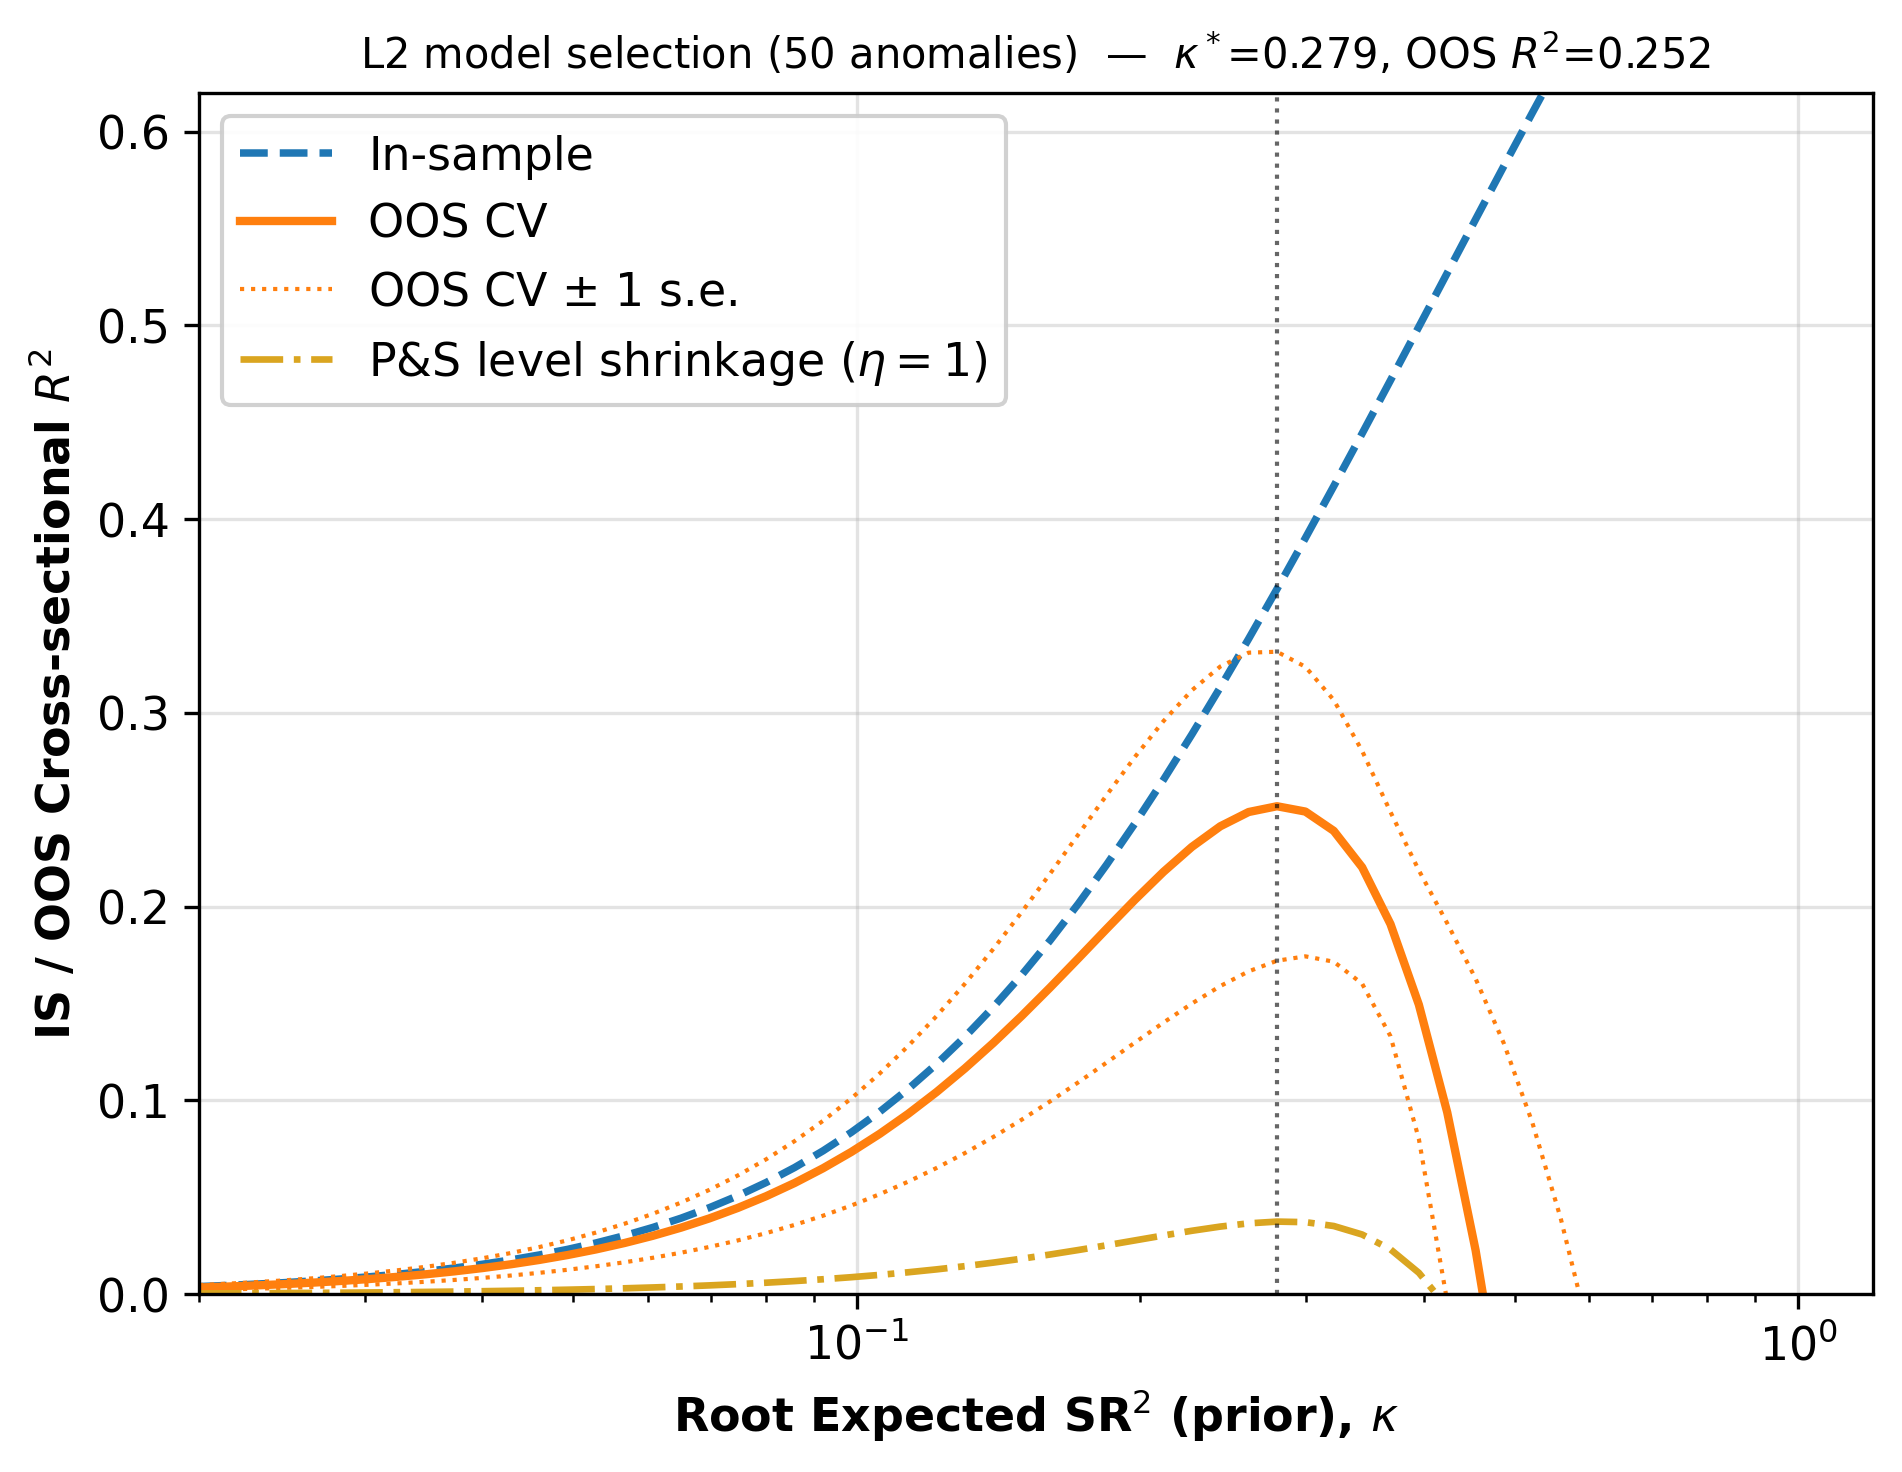
\includegraphics[width=0.74\textwidth]{fig1_l2_selection.png}
\caption{Figure 1 --- L2 model selection (paper Figure 4a). Relative shrinkage ($\eta{=}2$) peaks at OOS $0.252$;
literal level shrinkage ($\eta{=}1$, extension R4) tops out at only $0.063$, and its optimal penalty is about two
orders of magnitude stronger than that of relative shrinkage (the two humps sit on opposite sides), confirming that
``relative shrinkage is the key.''}\label{fig:fig1}
\end{figure}

\subsection{Figure 2 --- L1--L2 dual-penalty contours}
Figure~\ref{fig:fig2} is a two-panel heatmap: horizontal axis $\kappa$ (L2 strength), vertical axis the number of
nonzero coefficients (L1 sparsity, log scale), color the OOS $\Rtwo$. (a) For the raw 50 anomalies the high-scoring
region sits at a \textbf{high nonzero count} (it can hardly be made sparse); (b) for their principal components the
high-scoring region \textbf{extends down to very few nonzeros}. At $\le 10$ nonzeros the best OOS in PC space is
$0.233$ versus only $0.108$ in characteristics space. \textbf{This is the direct evidence that ``sparsity exists
only in PC space.''}

\begin{figure}[H]\centering
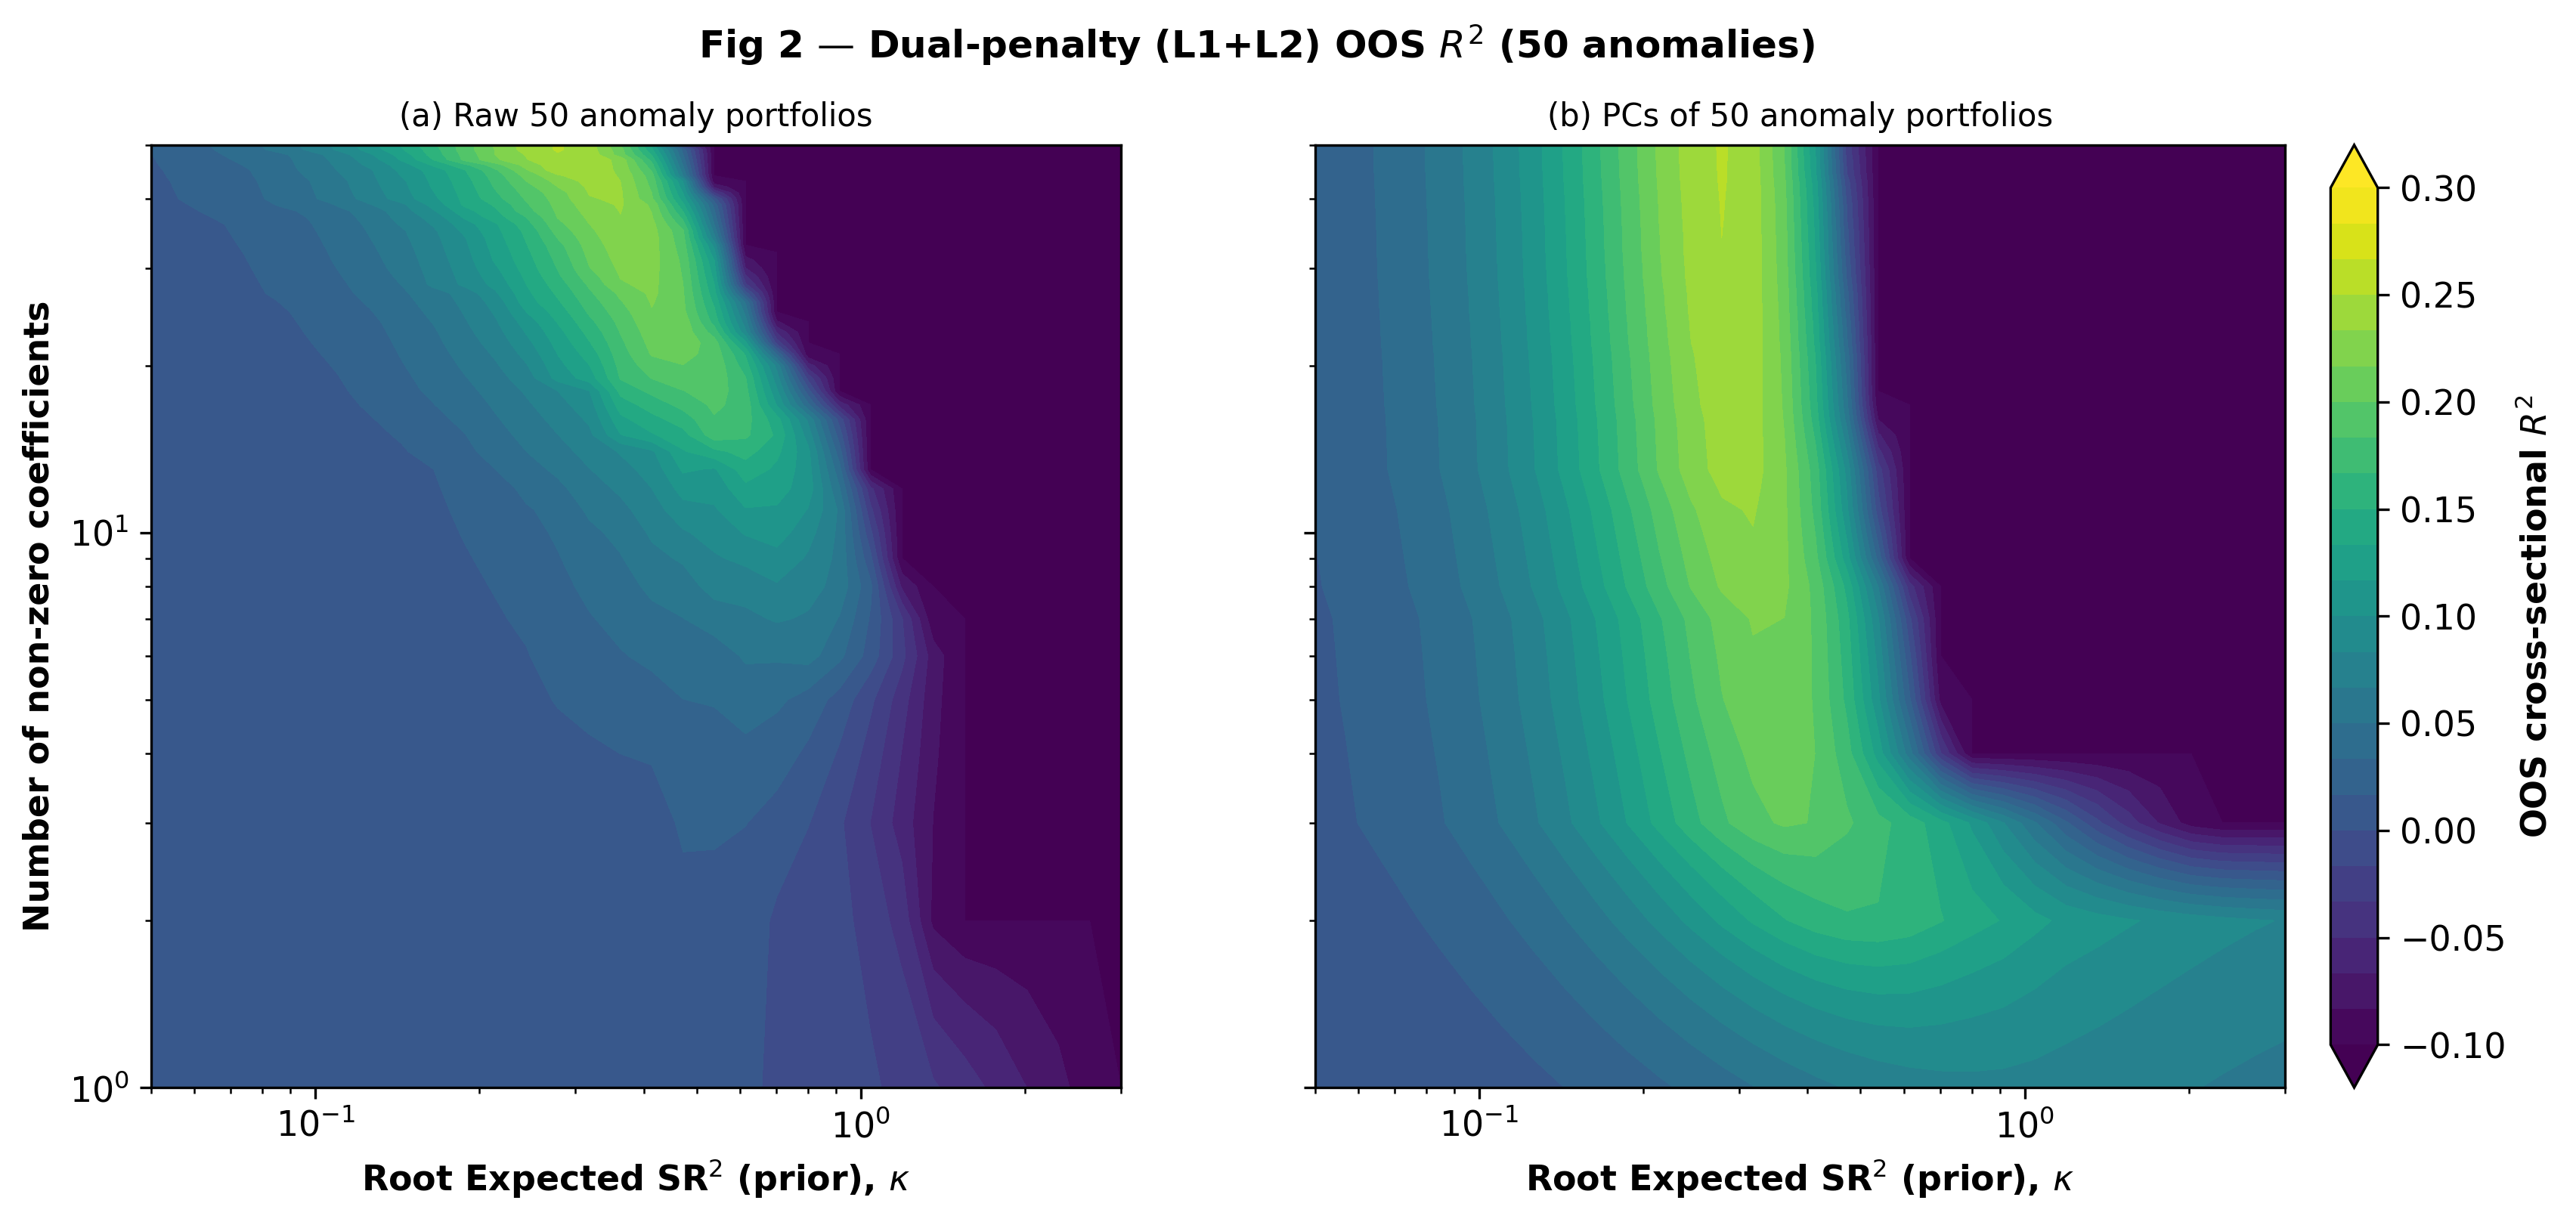
\includegraphics[width=0.92\textwidth]{fig2_dual_penalty_contour.png}
\caption{Figure 2 --- L1--L2 dual-penalty OOS $\Rtwo$ contours (paper Figure 3a/3b). Left: raw characteristics;
right: principal components. The high-scoring region extends to very few nonzeros in PC space but not in
characteristics space.}\label{fig:fig2}
\end{figure}

\subsection{Figure 3 --- distribution of SDF coefficients in PC space}
At the optimal $\kappa^*$ we rotate the SDF coefficients into PC space (eq.~\ref{eq:bpc}); Figure~\ref{fig:fig3}
shows the $|t|$ statistic of each PC. The largest are, in order, PC5, PC1, PC2, PC4, PC11, PC15, PC10\dots, which
matches the paper's Table 1b \textbf{almost item by item}. The large loadings tilt toward high-variance PCs, but
mid-variance PCs such as PC10/11/15 also carry sizable loadings --- \textbf{the information is spread over about
twenty PCs} rather than concentrated in the first few, exactly the basis on which the paper rejects
characteristics-sparsity in favor of PC shrinkage.

\begin{figure}[H]\centering
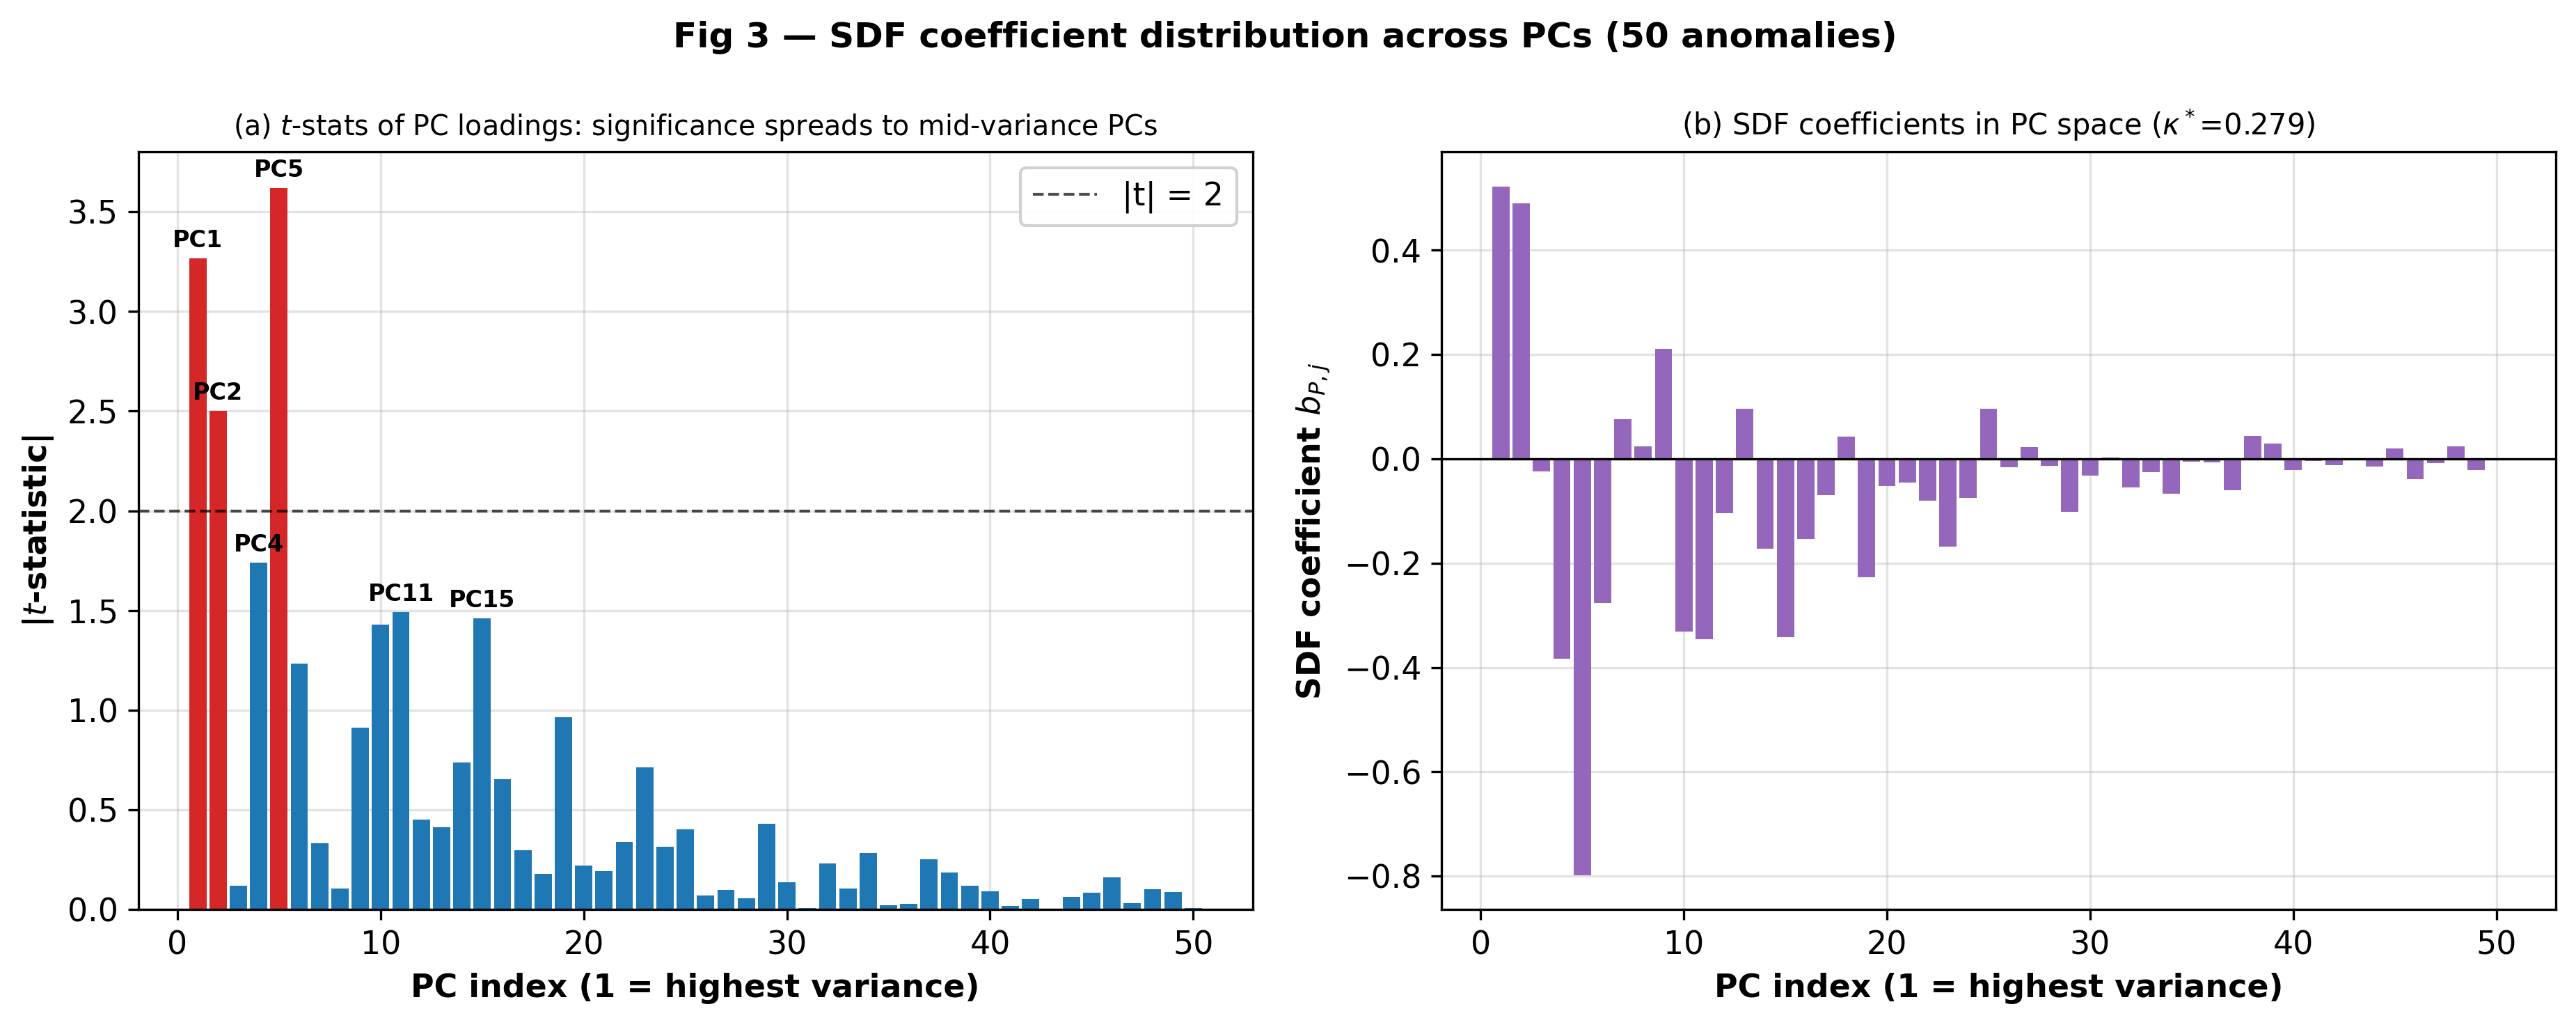
\includegraphics[width=0.86\textwidth]{fig3_pc_coefficients.png}
\caption{Figure 3 --- $|t|$ statistics and coefficients of the SDF in PC space at the optimal shrinkage
(paper Table 1b).}\label{fig:fig3}
\end{figure}

\subsection{Figure 4 --- sparse vs.\ dense}
In Figure~\ref{fig:fig4} the horizontal axis is the number of factors entering the SDF and the vertical axis is the
maximum OOS $\Rtwo$ attainable at that sparsity level when sweeping all L2 strengths (the ``ridge'' of the Figure 2
contours). \textbf{PCs rise quickly} (2 PCs $\to$ 0.17, 4 $\to$ 0.21, 10 $\to$ 0.23, near the maximum);
\textbf{characteristics rise slowly} (4 $\to$ 0.02; about 50 are needed to catch up). The OOS annualized Sharpe
ratio of the dense L2 model (50 factors) is markedly higher than that of the sparse L1 model (about 2 factors).
This is the most direct OOS evidence that ``characteristics-sparsity fails while PC-sparsity holds.''

\begin{figure}[H]\centering
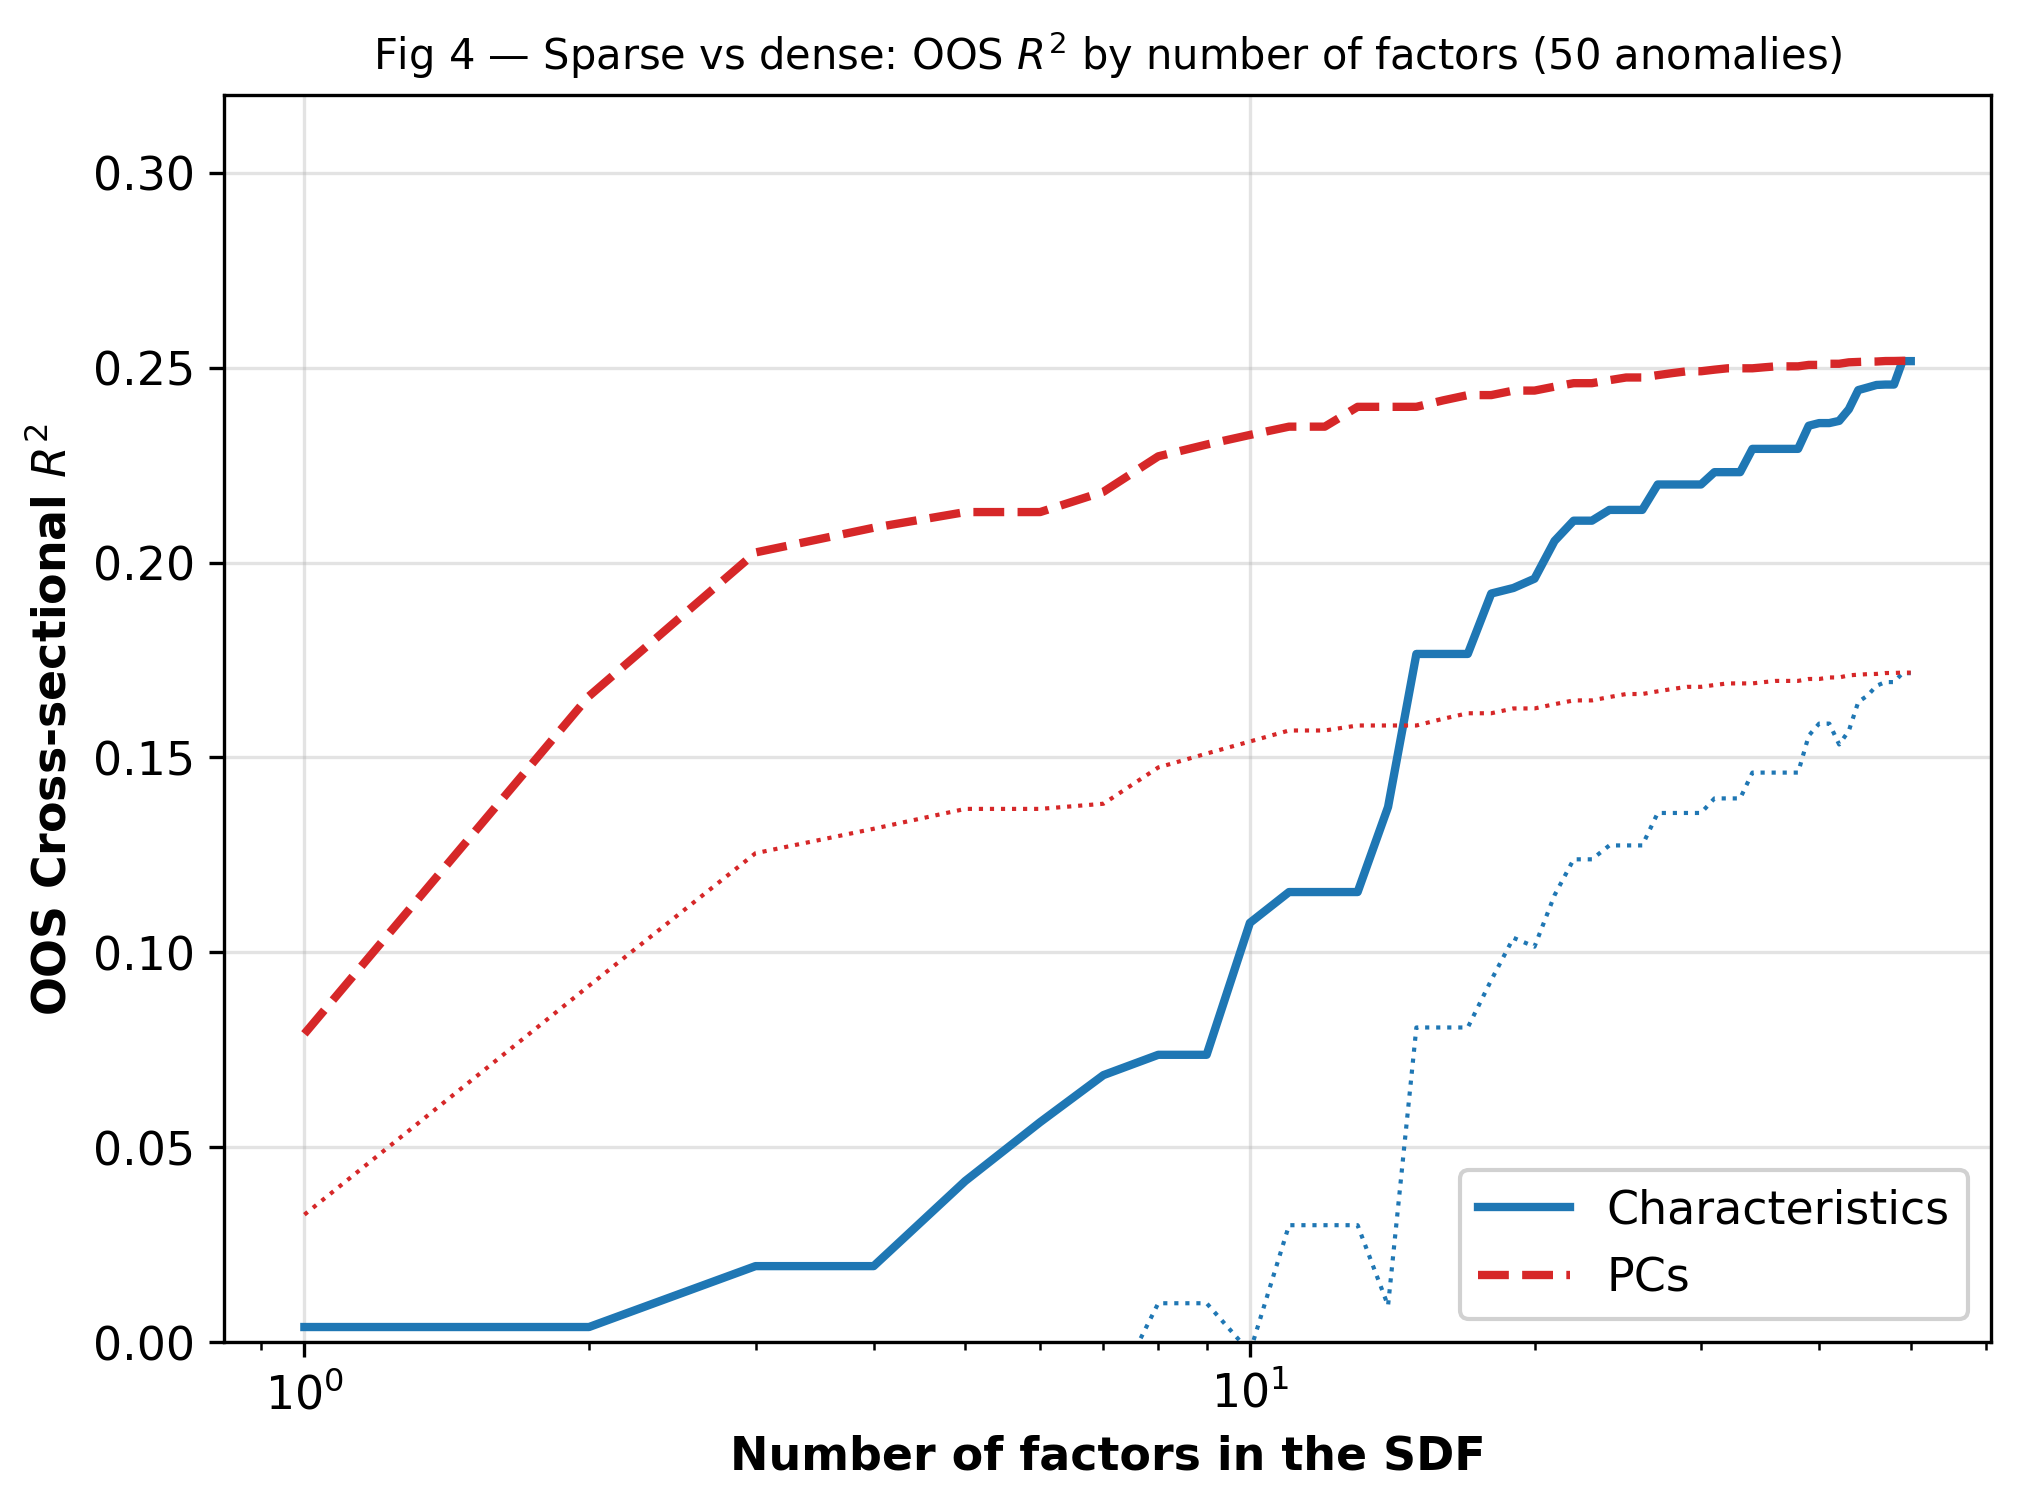
\includegraphics[width=0.70\textwidth]{fig4_sparsity_frontier.png}
\caption{Figure 4 --- sparse vs.\ dense OOS $\Rtwo$ (paper Figure 4b). The PC line saturates quickly; the
characteristics line rises slowly.}\label{fig:fig4}
\end{figure}

% ============================================================
\section{Machine-learning extension: a tiny MLP for nonlinear adaptive shrinkage}\label{sec:mlp}
% ============================================================
In PC space the paper's linear estimator is equivalent to a fixed shrinkage curve $w(d)=d/(d+\gamma)$. As the
first ``AI increment'' we replace it with an \textbf{adaptive penalty} $\gamma_j$ learned by a \textbf{tiny shallow
MLP} (1 hidden layer, 16 neurons, input $\log d_j$ only, trained by scipy L-BFGS with numerically checked analytic
gradients), evaluated under the exact same 3-fold OOS criterion as the four figures (the test block is fully held
out; the MLP is trained on an inner fit/validation split of the training block only, with no data leakage).

\textbf{Result (honest): the MLP does not win} --- linear ridge OOS $\Rtwo\approx0.22$ vs.\ the tiny MLP
$\approx0.07$ (Figure~\ref{fig:fig5}). This is not a tuning failure but a meaningful finding: SDF coefficients are
dominated by noise in the means and pricing information is diffuse, so what is needed is \textbf{strongly
structured shrinkage that cannot be over-optimized in sample}; giving the model extra nonlinear flexibility only
makes it under-shrink and hurts OOS performance. We did not tune the result to make the MLP win. Section~\ref{sec:ext}
reinforces this from the interpretable-knob angle.

\begin{figure}[H]\centering
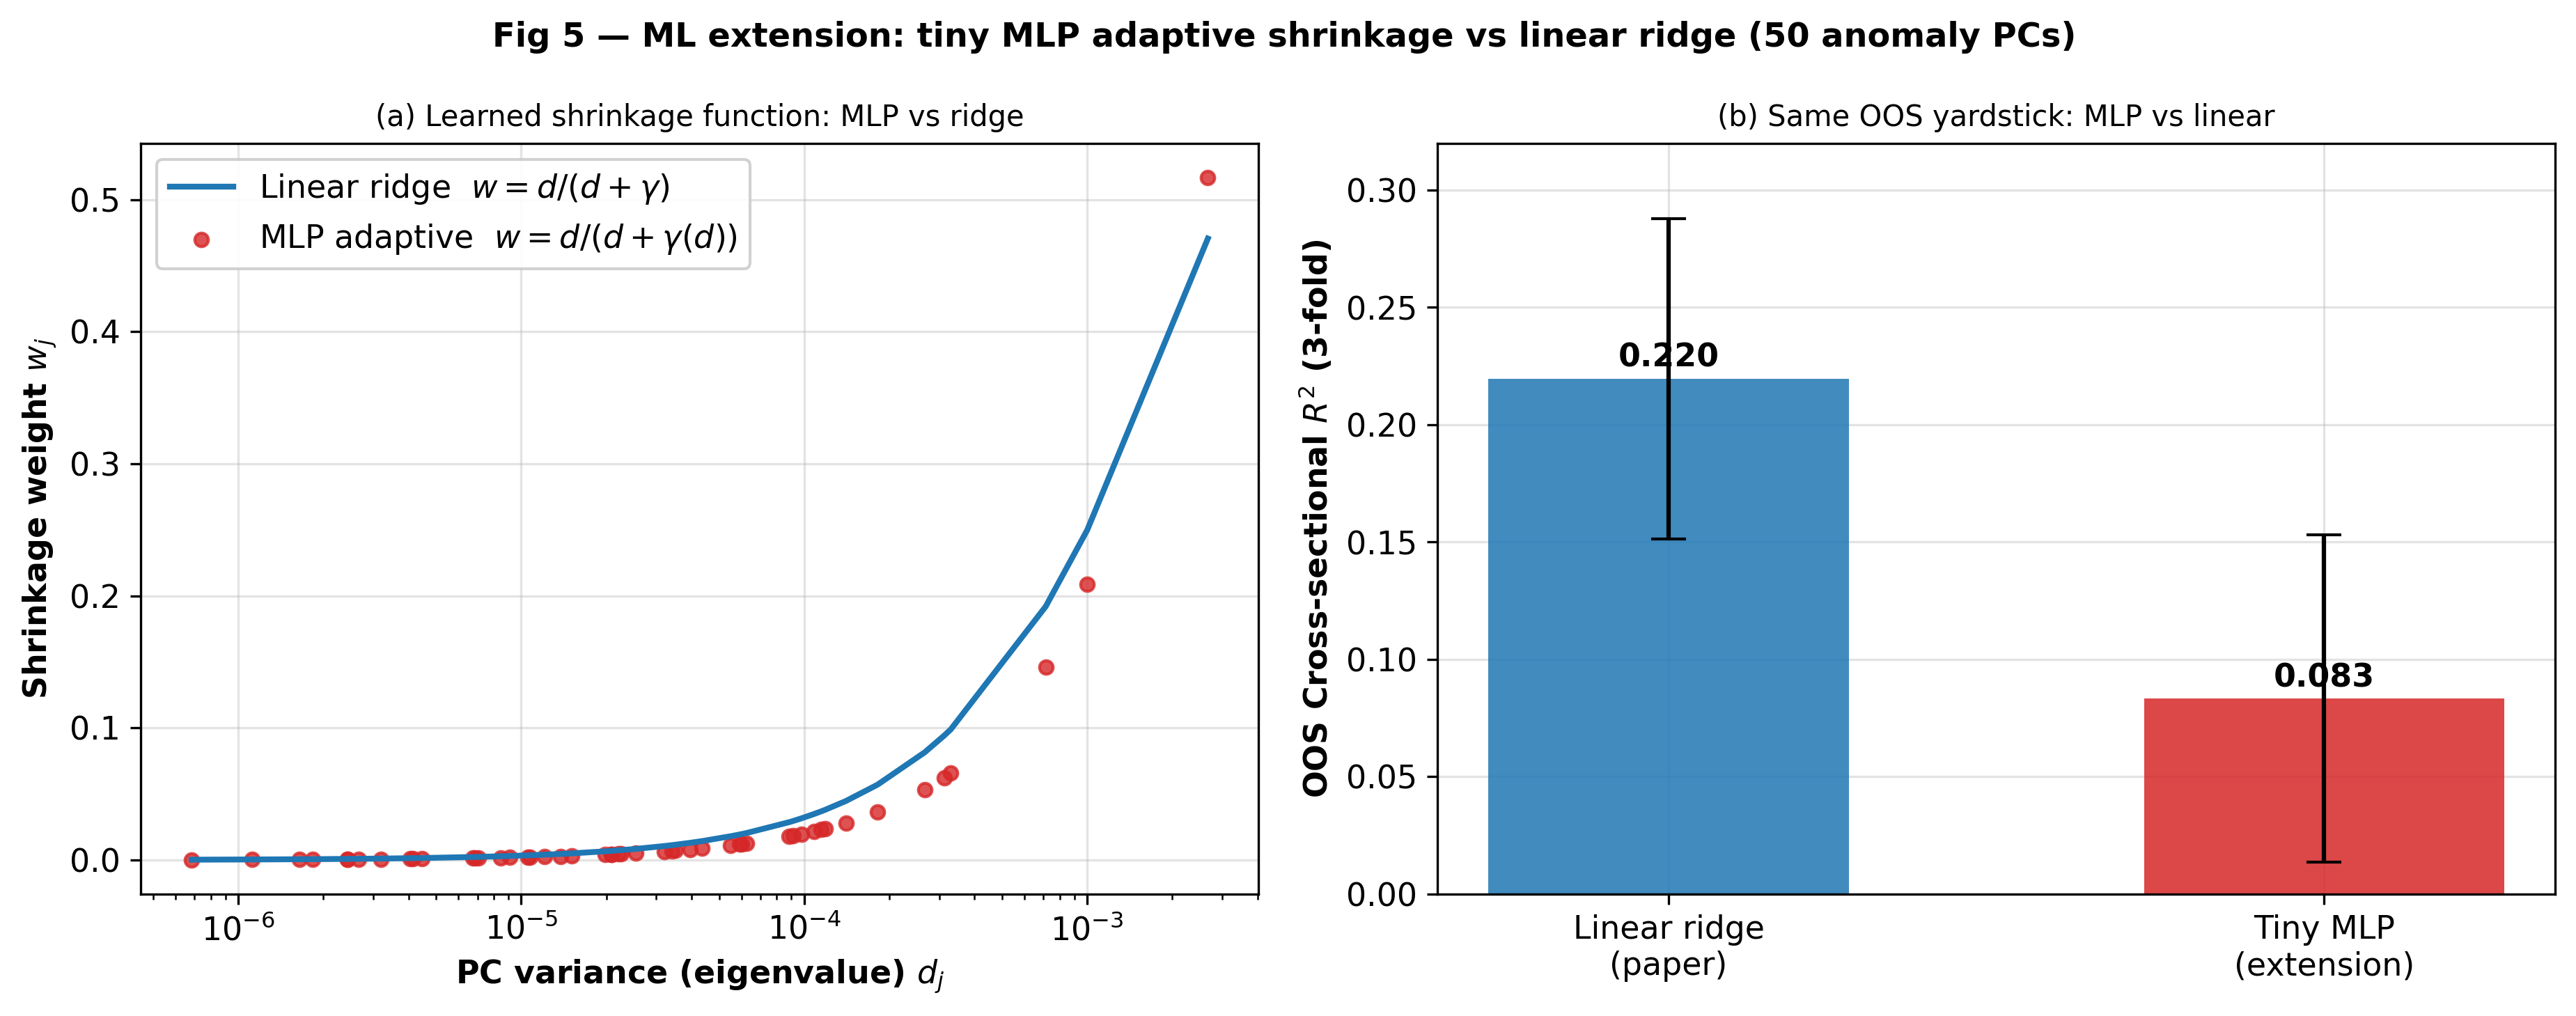
\includegraphics[width=0.86\textwidth]{fig5_mlp_extension.png}
\caption{Figure 5 --- tiny-MLP adaptive shrinkage vs.\ linear ridge. Left: the MLP's learned curve roughly tracks
ridge; right: OOS $\Rtwo$ comparison, with the MLP clearly no better than linear.}\label{fig:fig5}
\end{figure}

% ============================================================
\section{Extensions and robustness analyses}\label{sec:ext}
% ============================================================
This section presents our own work beyond the replication: five items, all CPU-only, seed-fixed, and folded into
the one-click reproduction.

\subsection{EXT --- generalized shrinkage curve: learning the shrinkage shape $\eta$}\label{sec:gen}
The paper \emph{fixes} $\eta{=}2$. We treat $\eta$ as a learnable ``shrinkage shape'' and jointly search
$(\eta,\gamma)$ under the exact same 3-fold OOS criterion as the four figures, asking whether giving the shrinkage
curve more flexibility can beat $\eta{=}2$. The shrinkage weight is $w_j(\eta,\gamma)$ from eq.~\eqref{eq:eta-weight},
itself a monotone shrinkage curve; each fold uses a train-only rotation (no look-ahead).

Figure~\ref{fig:fig7}(a) plots ``best OOS over $\gamma$'' against $\eta$: it rises steeply from $\eta{=}0$
(near-arbitrage, collapse), \textbf{forms a broad plateau over $\eta\in[3,4]$} (peak $\approx0.29$), and declines
gently for $\eta{>}4$ (approaching over-aggressive PC-sparsity). The learned $\eta^*\approx3.6$ gives OOS $0.292$,
a \textbf{$+0.04$ gain} over the paper's $\eta{=}2$ value of $0.252$. Figure~\ref{fig:fig7}(b) shows the learned
curve ($\eta^*$) is \emph{steeper} than $\eta{=}2$ --- the data prefer \emph{stronger} relative shrinkage of
low-variance PCs.

\textbf{Honest reading: this $+0.04$ gain is not statistically significant} (Section~\ref{sec:r3}; the 95\% CI of
$\Delta$ contains 0). Its meaning is twofold: (i) learning the shrinkage shape yields \textbf{no significant OOS
improvement}, i.e.\ \textbf{linear relative shrinkage is already near-optimal}, consistent with the MLP result of
Figure 5; (ii) if anything the data lean toward $\eta{>}2$ (\emph{stronger} relative shrinkage), which is
\textbf{aligned with and reinforces} the paper's economic argument ($\eta\ge2$, shrink low-variance PCs harder),
not a counterexample. The paper chooses $\eta{=}2$ as ``the smallest $\eta$ that keeps the portfolio weights
bounded''; our result shows $\eta{=}2$ sits on the left shoulder of a flat OOS plateau and is a robust, reasonable
choice.

\begin{figure}[H]\centering
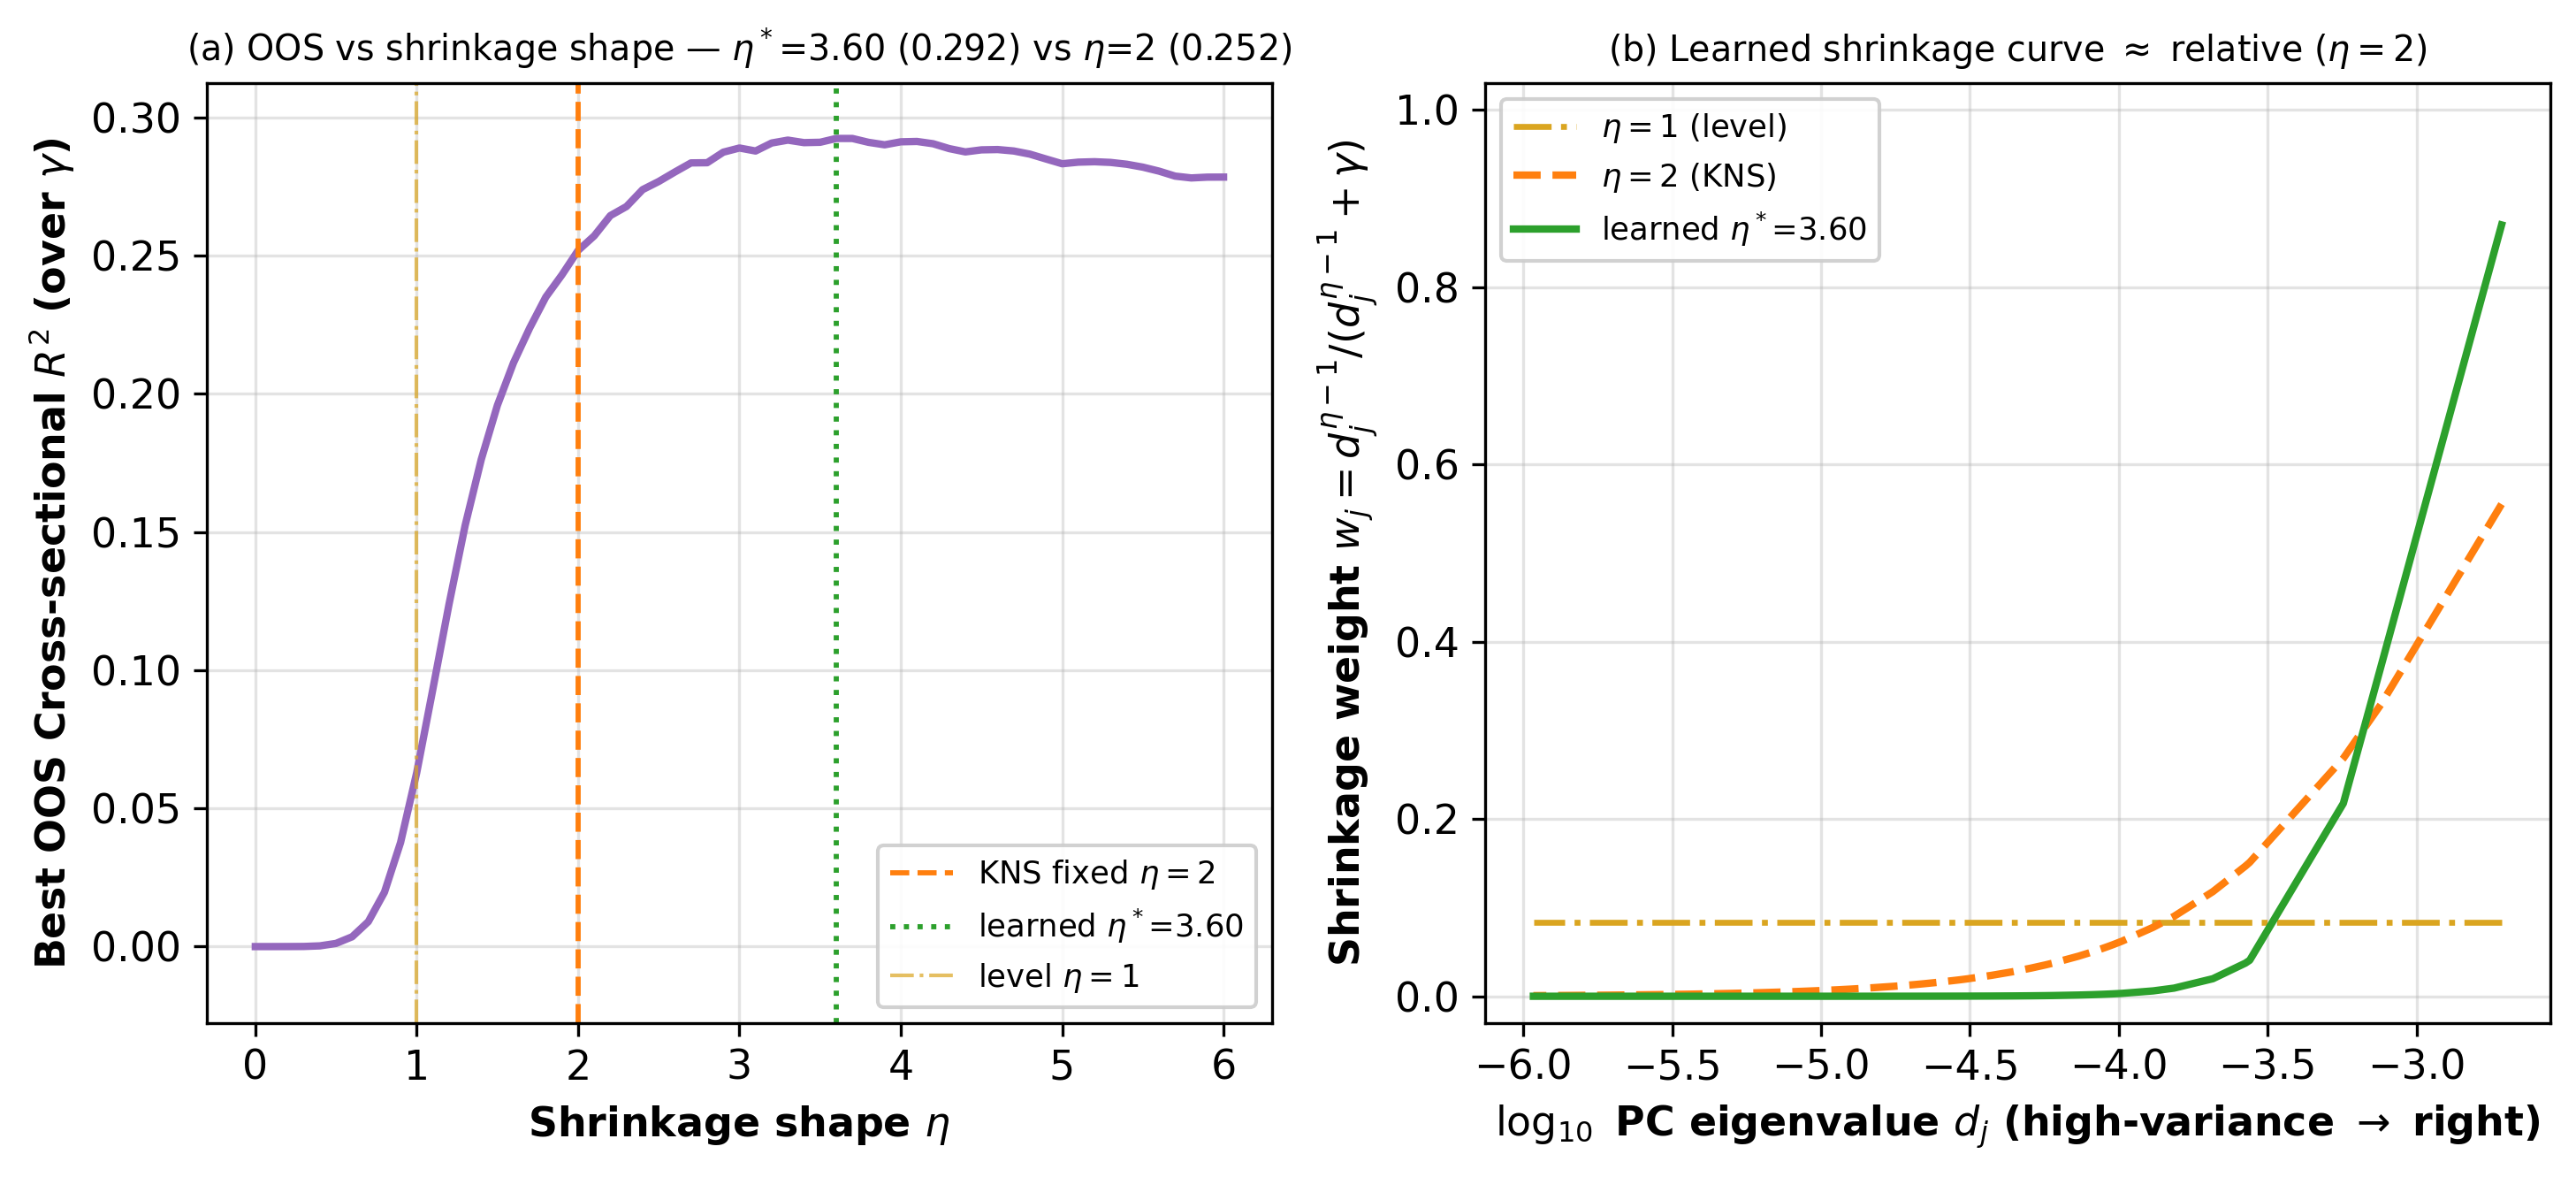
\includegraphics[width=0.96\textwidth]{fig7_generalized_shrinkage.png}
\caption{Figure 7 (EXT) --- generalized shrinkage curve. (a) Best OOS at each $\eta$: rise, broad plateau
($\eta^*{\approx}3.6$), gentle decline; (b) the learned curve $w(d)$ is steeper than $\eta{=}2$, but the two are
not significantly different out of sample (see R3).}\label{fig:fig7}
\end{figure}

\subsection{R4 --- the literal $\eta{=}1$ Pástor--Stambaugh benchmark}\label{sec:r4}
Pástor--Stambaugh (2000) corresponds to $\eta{=}1$ level (equal) shrinkage. Using the \textbf{literal $\eta{=}1$
posterior} $\hat b_{P,j}=\bar\mu_{P,j}/(d_j(1+\gamma))$ from eq.~\eqref{eq:eta-weight}, we replace the original
repo's level-shrinkage reparametrization and overlay it on Figure~\ref{fig:fig1}. Because the natural penalty
scales of level and relative shrinkage differ by about two orders of magnitude (their optimal humps sit on opposite
sides of the $\kappa$ axis --- exactly the paper's footnote that ``the $x$-axis is no longer $\kappa$ under
$\eta{=}1$''), we sweep level shrinkage over \emph{its own} penalty range to its optimum: \textbf{the best is only
$\Rtwo_{\text{oos}}=0.063$}, about one quarter of relative shrinkage's $0.252$. This is more principled than the
original repo's reparametrized version ($0.038$) and the qualitative conclusion is unchanged: \textbf{equal
shrinkage is far worse than relative shrinkage}.

\subsection{R3 --- block-bootstrap confidence intervals}\label{sec:r3}
We attach 95\% confidence intervals to the key OOS numbers via a \textbf{leakage-free circular block bootstrap}
(block length 21 trading days, preserving serial correlation). \emph{A methodological lesson:} naively
``resampling the whole series and then splitting into CV folds'' lets the same original observation land in both
the train and test folds, causing leakage (empirically inflating the OOS to $\sim0.8$); the correct approach is to
\textbf{resample independently within each fold's train and test windows} (which are disjoint, hence leakage-free).
The results (Table~\ref{tab:boot}):
\begin{itemize}
  \item $\eta{=}2$ relative shrinkage OOS $=0.252$, \textbf{95\% CI $[0.014,\,0.377]$, significantly above 0} ---
  shrinkage itself genuinely works.
  \item The EXT gain $\Delta=\Rtwo(\eta^*{=}3.6)-\Rtwo(\eta{=}2)$ has 95\% CI $=[-0.080,\,+0.109]$, \textbf{which
  contains 0 and is not significant} --- confirming ``learning the shrinkage shape yields no significant
  improvement; $\eta{=}2$ is near-optimal.''
\end{itemize}
The intervals are wide (estimating cross-sectional means is precisely the most fragile step the paper emphasizes),
honestly reflecting the intrinsic uncertainty of out-of-sample pricing.

\begin{table}[H]\centering\small
\caption{Block-bootstrap confidence intervals (50 anomalies, $n_{\text{boot}}{=}300$, block length 21)}\label{tab:boot}
\begin{tabular}{lcc}
\toprule
Model & Point OOS $\Rtwo$ & 95\% CI \\
\midrule
$\eta{=}1$ (level) & $0.063$ & $[-0.001,\ 0.219]$ \\
$\eta{=}2$ (relative, KNS) & $0.252$ & $[0.014,\ 0.377]$ \\
$\eta^*{=}3.6$ (learned) & $0.292$ & $[0.034,\ 0.411]$ \\
\midrule
Gain $\Delta=\Rtwo(\eta^*)-\Rtwo(\eta{=}2)$ & $+0.040$ & $[-0.080,\ +0.109]$ (contains 0) \\
\bottomrule
\end{tabular}
\end{table}

\subsection{R2 --- removing look-ahead: a train-only PC rotation}\label{sec:r2}
The replication backbone rotates factors into PC space using the eigenvectors $Q$ of the \textbf{full-sample}
covariance, so the training block ``sees'' a $Q$ estimated partly from the test block --- a mild look-ahead. We
quantify it rigorously, with the conclusion splitting into two cases (Figure~\ref{fig:fig8}):
\begin{itemize}
  \item \textbf{Pure L2 ridge} (the Figure 1 backbone, the L2 envelope of Figure 4): under the isotropic penalty
  $\gamma I$, ridge is \emph{rotation-equivariant}, so the OOS $\Rtwo$ is \textbf{exactly independent} of the
  choice of $Q$ --- the difference between full-sample $Q$ and train-only $Q$ is $3.3\times10^{-15}$
  (machine precision, i.e.\ exactly 0).
  \item \textbf{PC-sparse} (L1 selection of PCs, rotation-dependent): comparing the \emph{global maximum} OOS of
  the two versions, train-only $Q$ gives $0.269$, which is \emph{no lower} than full-sample $Q$'s $0.252$ ---
  \textbf{the look-ahead does not inflate the backbone PC results}; if anything they rise slightly once it is removed.
\end{itemize}
Moreover, the generalized shrinkage curve of Section~\ref{sec:gen} (and the $\eta{=}1$ curve of Figure 1)
\textbf{already use train-only $Q$ by default}, so they have no such look-ahead. The paper's PC conclusions are
therefore robust to removing look-ahead.

\begin{figure}[H]\centering
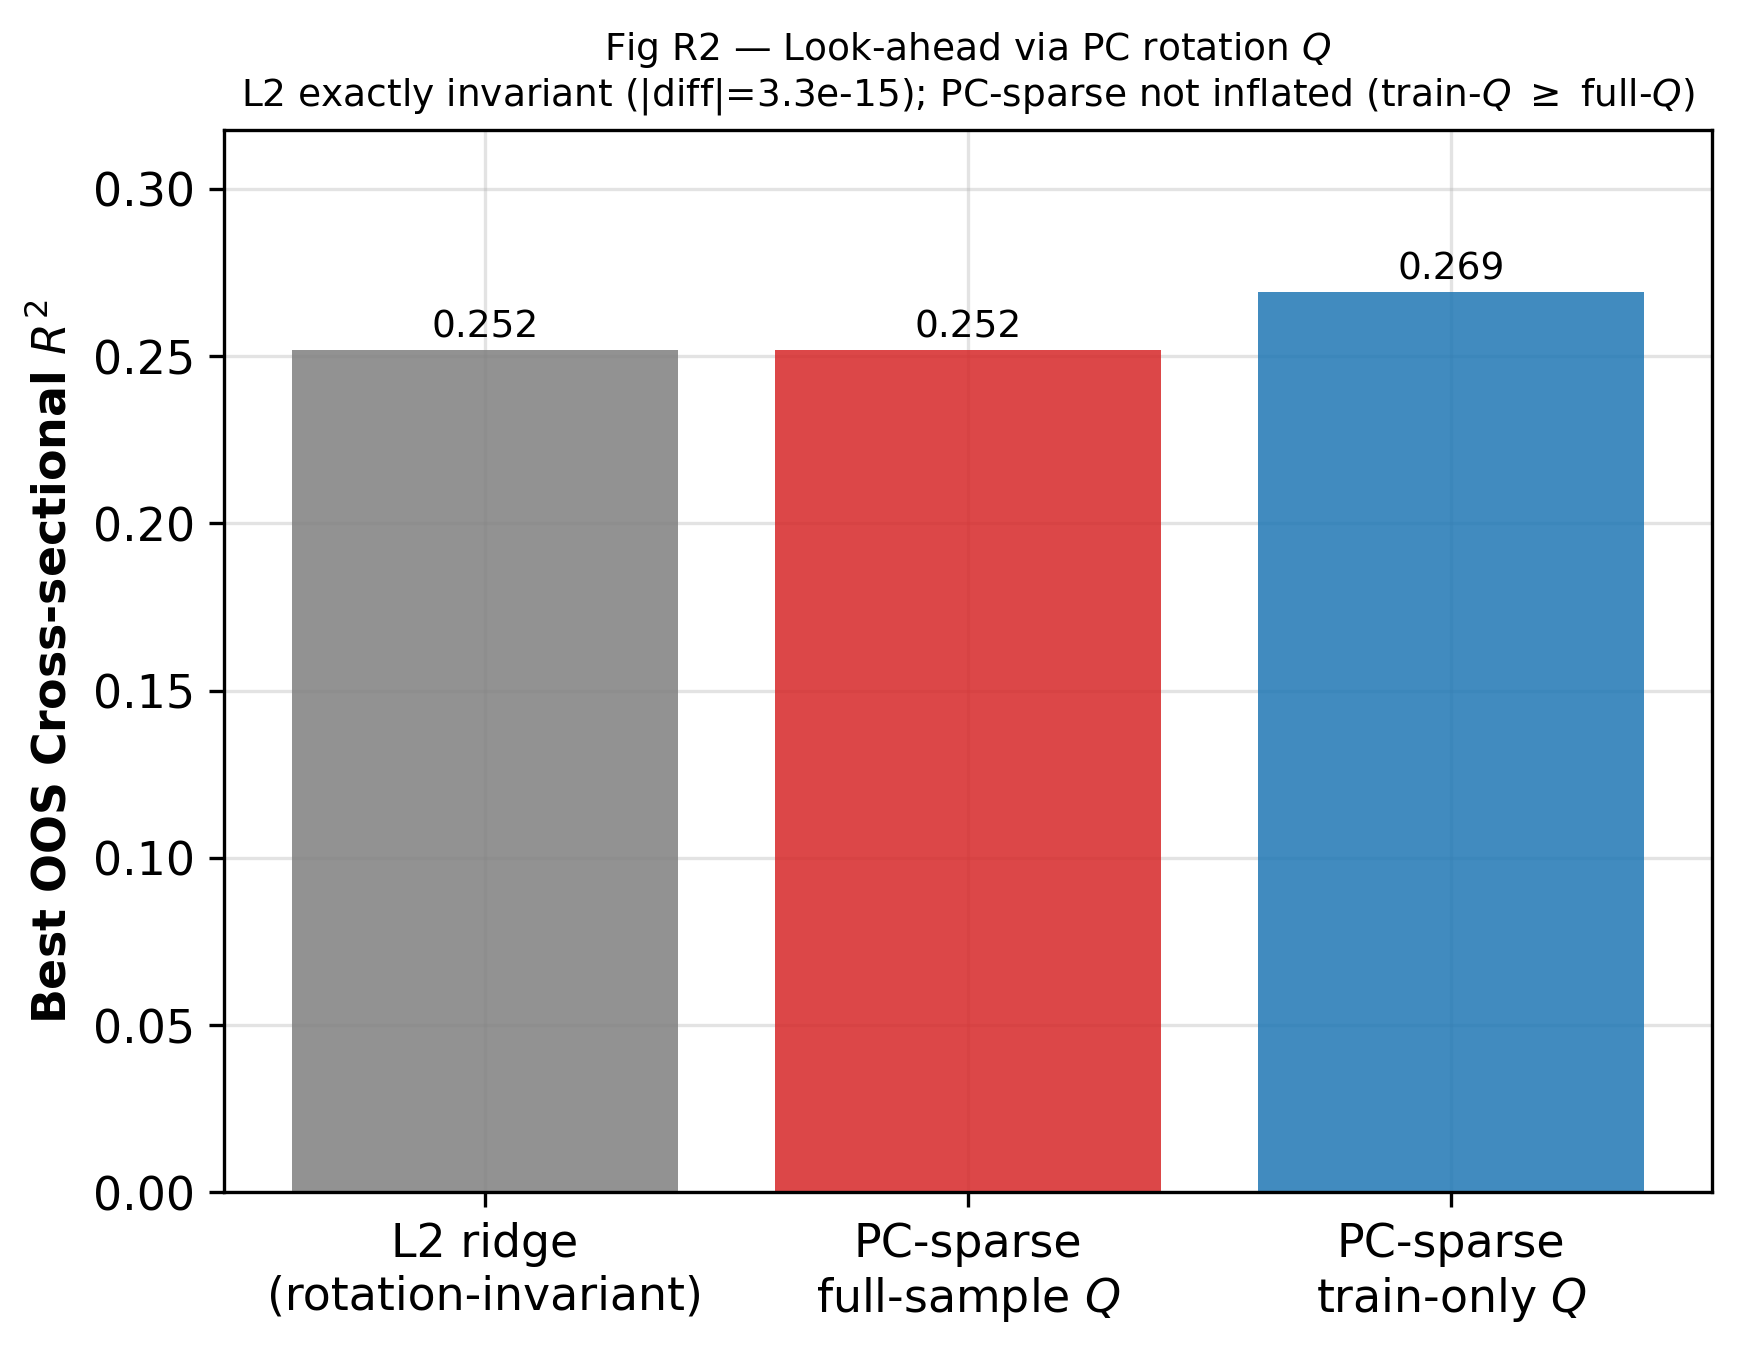
\includegraphics[width=0.58\textwidth]{fig8_r2_lookahead.png}
\caption{Figure 8 (R2) --- look-ahead via the PC rotation $Q$. Pure L2 is rotation-invariant (difference
$\sim10^{-15}$); the PC-sparse global optimum under train-only $Q$ is no lower than under full-sample $Q$, so the
backbone results are not inflated.}\label{fig:fig8}
\end{figure}

\subsection{R1 --- FF25 preliminary analysis (a negative control and low-dimensionality)}\label{sec:r1}
The paper's Section 4.1 uses FF25 --- a low-dimensional ``known-answer'' setting --- to check that the method
recovers an SMB/HML-like few-factor SDF. We run the \textbf{exact same} KNS pipeline as for the 50 anomalies on
FF25 (same 1963--2017 window) and find (Figure~\ref{fig:fig6}):
\begin{itemize}
  \item (a) FF25 is \textbf{lower-dimensional} --- the top 3 PCs account for 65\% of the variance (the 50 anomalies
  are more spread out), consistent with the paper's use of it as a low-dimensional warm-up.
  \item (b) But after de-marketing, the \textbf{residual cross-section has OOS $\Rtwo\approx0$} (with large standard
  errors): the size/value residual premia are strongly time-varying and are almost unpredictable out of sample
  under a 3-fold time split.
\end{itemize}
This is a valuable \textbf{negative control}: the same pipeline honestly returns about 0 when there is \emph{no
stable signal}, which argues that the $0.25$ on the 50 anomalies \textbf{is not a mechanical artifact}. It also
shows that the OOS value of the KNS method appears \textbf{specifically in the high-dimensional anomaly
cross-section}, not in the classic low-dimensional FF25 --- in line with the paper's premise that the
``multidimensional challenge'' bites only in high dimensions.

\begin{figure}[H]\centering
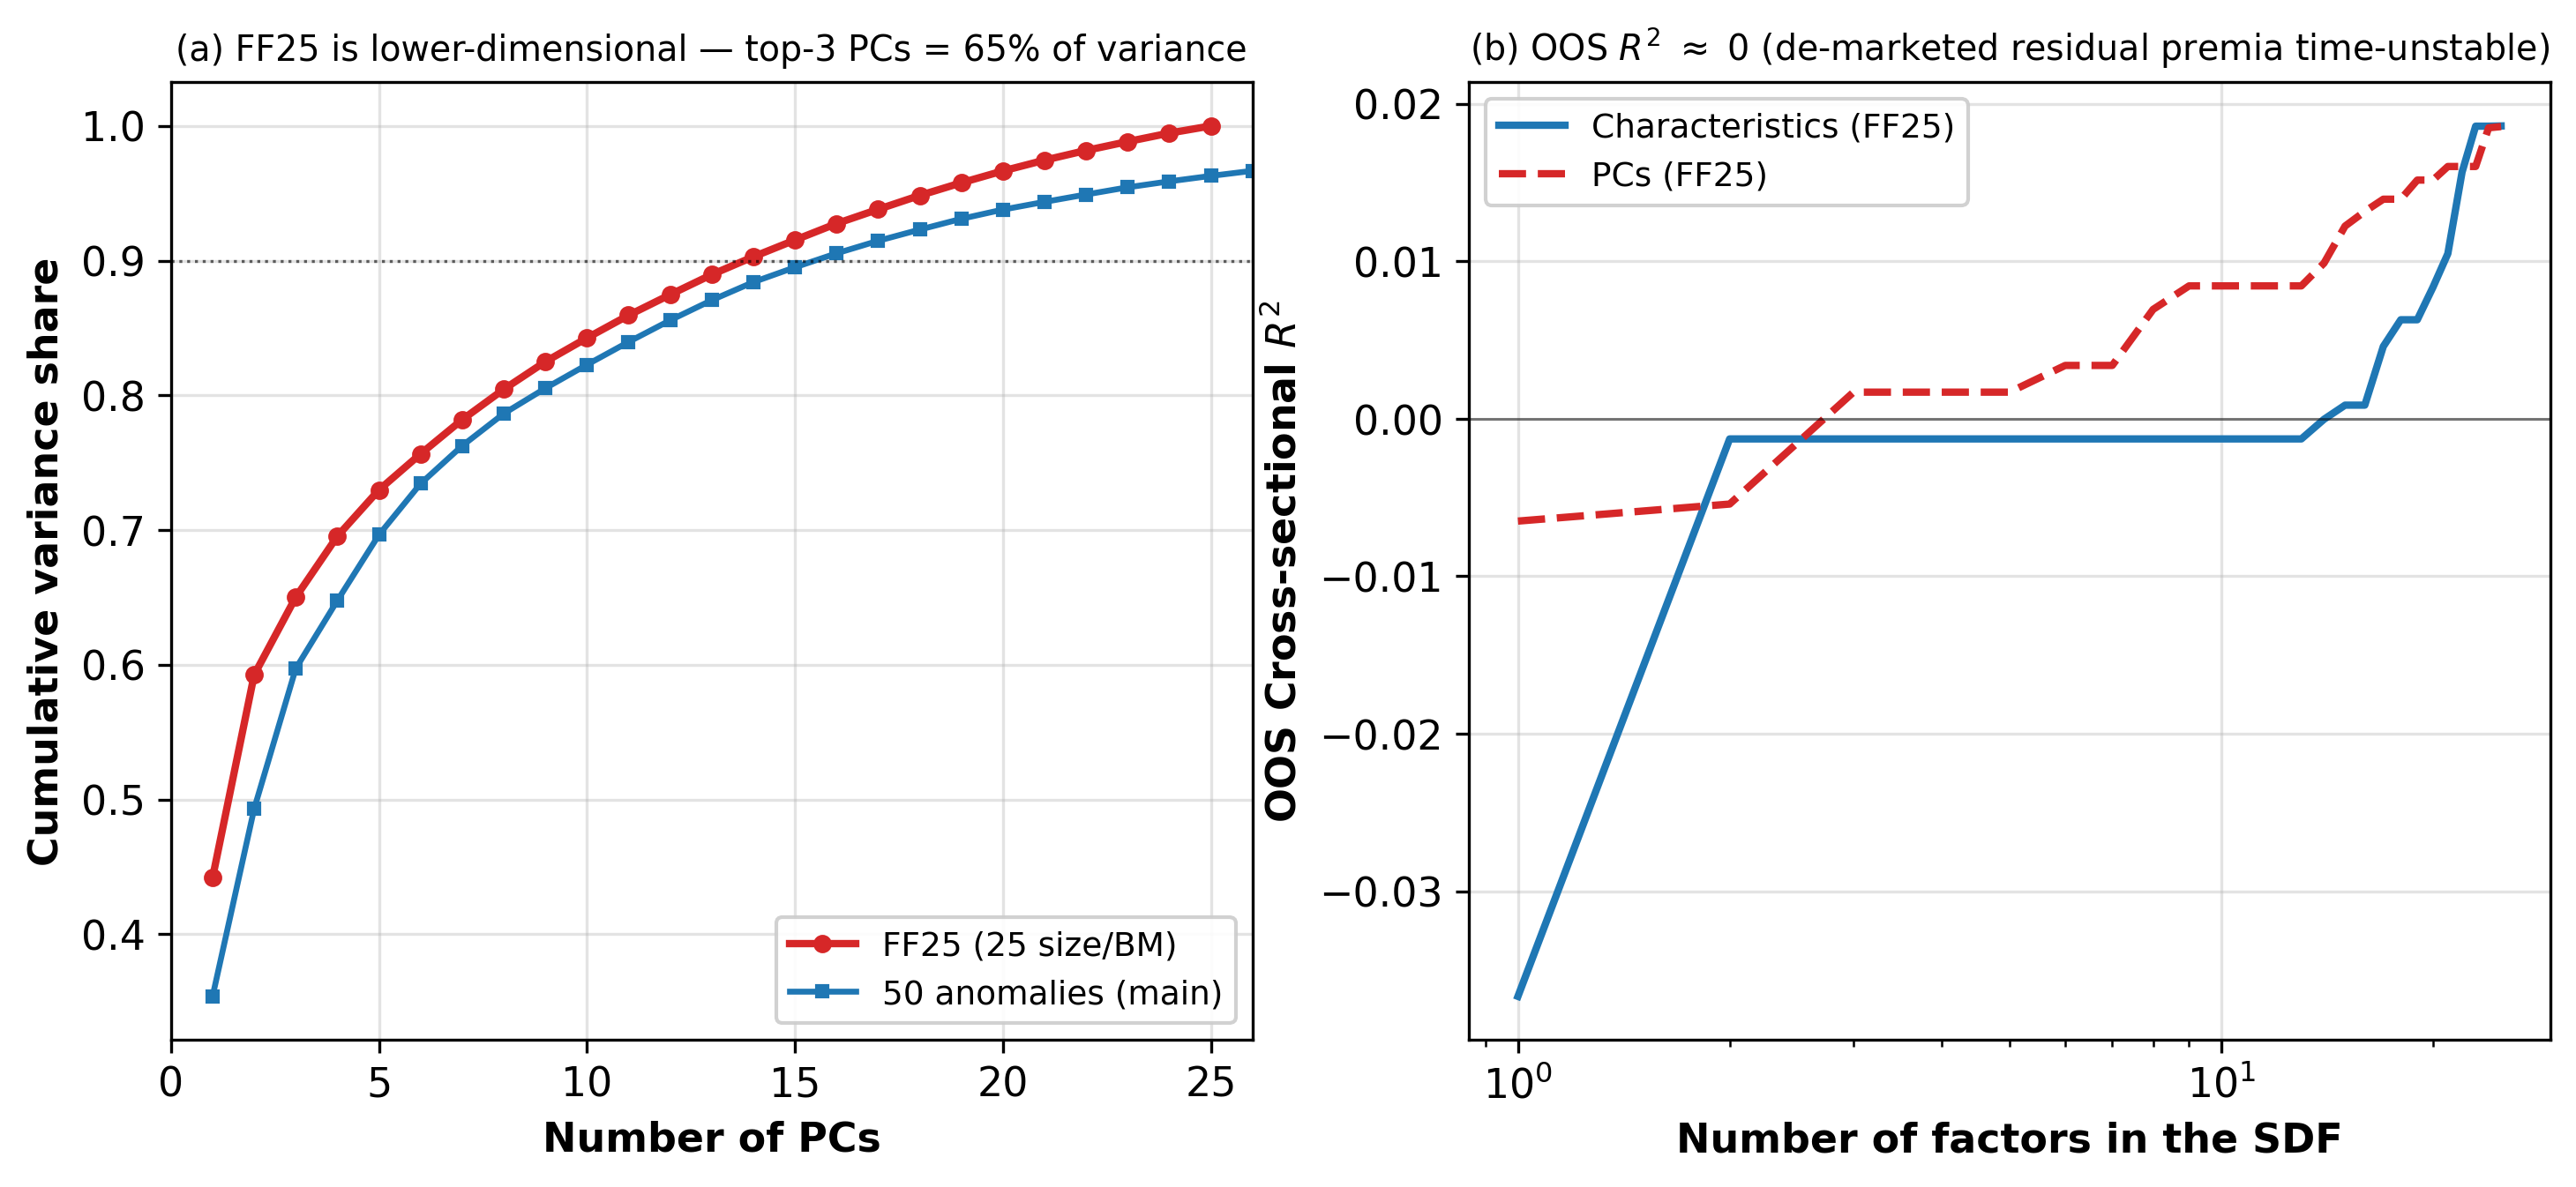
\includegraphics[width=0.96\textwidth]{fig6_ff25_sparsity.png}
\caption{Figure 6 (R1) --- FF25 preliminary analysis. (a) FF25 is lower-dimensional than the 50 anomalies
(cumulative variance); (b) the de-marketed residual cross-section has OOS $\Rtwo\approx0$ (time-varying premia),
serving as a negative control.}\label{fig:fig6}
\end{figure}

% ============================================================
\section{Known limitations}
% ============================================================
\begin{itemize}
  \item \textbf{Full-sample $\beta$ in de-marketing}: consistent with the paper's own approach; a mild look-ahead,
  but very stable given the large daily sample.
  \item \textbf{The PC coefficients of Figure 3} are an in-sample descriptive quantity at the optimal $\kappa^*$,
  whose PC rotation uses the full-sample $Q$ (descriptive, inherent).
  \item \textbf{The bootstrap intervals are wide}: only 3 folds plus large noise in estimating cross-sectional
  means; this is an honest reflection rather than a defect.
  \item \textbf{$\eta^*\approx3.6$ is near the upper end of the search}: we extended the grid to $\eta\in[0,6]$ to
  confirm the plateau and the decline, so $\eta^*$ is not a grid-boundary artifact; but the plateau is flat and the
  precise value of $\eta^*$ is not sharply identified (hence its gain over $\eta{=}2$ is not significant).
  \item \textbf{No paid data}: we cannot reproduce the paper's ultra-high-dimensional dataset of thousands of
  characteristic interactions; the main 50-anomaly set already supports all qualitative conclusions.
\end{itemize}

% ============================================================
\section{Division of labor}
% ============================================================
This is \textbf{Group 3}; the members and the division of labor are as follows.

\begin{table}[H]\centering\small
\caption{Group members and division of labor (Group 3)}
\begin{tabular}{p{3.4cm} p{3.2cm} p{8.0cm}}
\toprule
Name (ID) & Major & Main responsibilities \\
\midrule
\memberA~(\sidA) & \majorA & Programming and implementation: all code (the unified numerical core, the four core
figures, and the five extensions), the figures, the one-click reproduction pipeline, and the self-tests. \\
\addlinespace
\memberB~(\sidB) & \majorB & Theoretical derivations: the shrinkage prior, the general-$\eta$ posterior and
shrinkage weight, and the level-vs.-relative shrinkage argument. \\
\bottomrule
\end{tabular}
\end{table}
\noindent Completed jointly by both members: the literature review of the original paper, the selection of the
extension directions, and the writing of this report.

% ============================================================
\section{Reproducibility and environment}
% ============================================================
\textbf{Hard constraints respected}: CPU-only, no GPU/CUDA; no paid data (only portfolio-level returns plus freely
available Ken French data); dependencies limited to \texttt{numpy / pandas / matplotlib / scipy}; fixed random
seeds (\texttt{np.random.seed(0)} / \texttt{default\_rng(0)}).

\textbf{One-click reproduction} (about 2 minutes, producing Figures 1--8 in \texttt{outputs/}):
\begin{verbatim}
    uv sync                          # install dependencies
    uv run python reproduce_all.py   # four core figures + MLP + five extensions (Fig. 1-8)
    uv run python _selftest_core.py  # numerical self-tests (6 checks, incl. general-eta guards)
\end{verbatim}
Environment: Python 3.14, numpy 2.4, pandas 3.0, matplotlib 3.10, scipy 1.17 (versions locked in \texttt{uv.lock} /
\texttt{requirements.txt}). Code layout: \texttt{scs\_core} (numerical core, incl.\ the unified general-$\eta$
OOS-CV), \texttt{scs\_data} (unified data pipeline, incl.\ \texttt{prepared\_ff25}), \texttt{dual\_penalty}
(dual-penalty sweep, incl.\ the train-$Q$ option), \texttt{fig1--4} (core figures), \texttt{mlp\_sdf} (Figure 5),
\texttt{gen\_shrinkage} (Figure 7), \texttt{r2\_lookahead} (Figure 8), \texttt{bootstrap\_ci} (R3), and
\texttt{fig6\_ff25\_sparsity} (Figure 6).

% ============================================================
\begin{thebibliography}{9}
\small
\bibitem{kns2020} Kozak, S., Nagel, S., \& Santosh, S. (2020). Shrinking the cross-section.
\emph{Journal of Financial Economics}, 135(2), 271--292.
\bibitem{kns2018} Kozak, S., Nagel, S., \& Santosh, S. (2018). Interpreting factor models.
\emph{Journal of Finance}, 73(3), 1183--1223.
\bibitem{ps2000} Pástor, \v{L}., \& Stambaugh, R. F. (2000). Comparing asset pricing models: An investment perspective.
\emph{Journal of Financial Economics}, 56(3), 335--381.
\bibitem{ff1993} Fama, E. F., \& French, K. R. (1993). Common risk factors in the returns on stocks and bonds.
\emph{Journal of Financial Economics}, 33(1), 3--56.
\bibitem{zou2005} Zou, H., \& Hastie, T. (2005). Regularization and variable selection via the elastic net.
\emph{Journal of the Royal Statistical Society B}, 67(2), 301--320.
\bibitem{lw2004} Ledoit, O., \& Wolf, M. (2004). A well-conditioned estimator for large-dimensional covariance matrices.
\emph{Journal of Multivariate Analysis}, 88(2), 365--411.
\bibitem{hj1991} Hansen, L. P., \& Jagannathan, R. (1991). Implications of security market data for models of dynamic economies.
\emph{Journal of Political Economy}, 99(2), 225--262.
\end{thebibliography}

\end{document}
